\subsection{Implied Read Orders - A road to optimality?}

    %State examples showing that implied write orders though sorted can still have us explore more executions.
    %Take pics from notes.
    Let us start with the example below:
    \begin{figure}
        \centering
        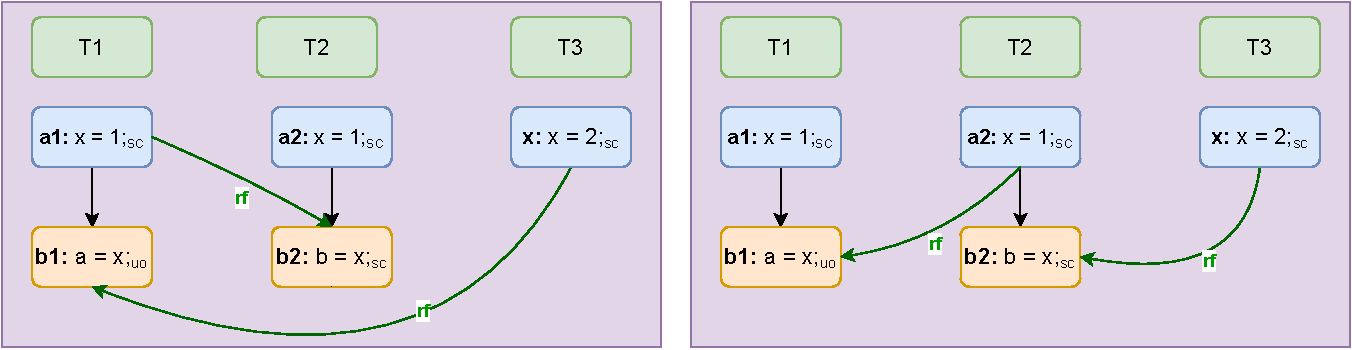
\includegraphics{Equivalence_Example.pdf}
        \caption{Example program for read orders}
        \label{read_ord:ex1}
    \end{figure}

    Consider now two possible execution graphs of the above program as below:
    \begin{figure}
        \centering
        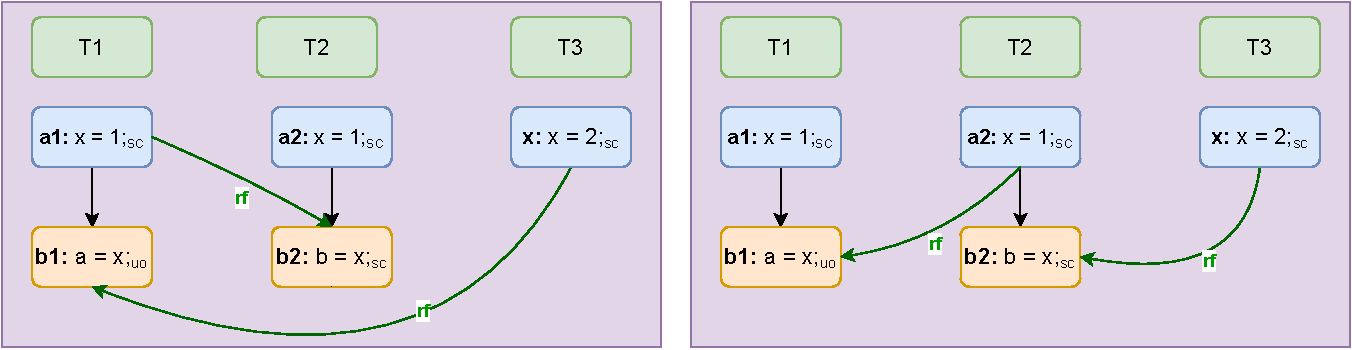
\includegraphics{Equivalence_Example.pdf}
        \caption{Two execution graphs of the program in Figure \ref{read_ord:ex1}}
        \label{read_ord:exec_ex1}
    \end{figure}

    Notice that both the above executions respect the irreflexivity constraint Prop \ref{prop1}.
    Naturally, we must then consider both executions while performing model checking.
    However, also notice that, on swapping threads $T_1$ and $T_3$ of the first execution graph, we do obtain the second execution graph.
    This, by our definition of symmetry would mean both the above executions are symmetric. 

    %Explain why the above symmetry exists.
    The only difference that is present in the two executions is from where the read values of $T_1$ and $T_3$ come from.
    In particular, note that $T_1$'s read value comes from the write of $T_4$, whereas that of $T_3$ comes from $T_2$.
    This by the standards of sequential consistency implies that $T_3$'s read occurred before that of $T_1$.
    While in that of the second execution, the order of reads is reverse. 
    We can then conclude that we could leverage the read orders to even further reduce the set of executions we need to verify.  

    %Using them, note the reader that implied read orders are incorrect in some and so sorting them might help.
    The above examples show us that read orders can also play a role in defining symmetric executions.
    The question however, is whether we can resolve all these read orders while also keeping the implied write orders to respect Prop \ref{prop1}.
    For this, we define a notion of a state, which represents the set of implied write orders and implied read orders that exist.    

    \paragraph{Resolving implied Read orders}

        It is important to note that we consider resolving implied read orders only when all the implied write orders are resolved.
        This means, if any implied write orders do not respect Prop \ref{prop1}, then we only concern ourselves to resolving them.
        Our definition of implied read orders is only to capture those patterns in executions where Prop \ref{prop1} is satisfied.
        
        %total order between reads of symmetric threads.
        \begin{definition}{Symmetric Read Order ($sro$)}
            \label{SymReadOrd}
            A strict partial order between reads of symmetric threads.
            
            Consider a set of symmetric threads $T_1 \equiv T_2 \equiv ... \equiv T_n$. 
            Each of these threads have exactly one read event, and multiple write events, all to the same memory, say $x$. 
            Then each read in the above threads are involved in a symmetric order, such that
            \begin{align*}
                \forall i \in [0, n-1] \ . \ \reln{r_i}{sro}{r_{i+1}}.
            \end{align*}

        \end{definition}

        %definition of implied read order. 
        \begin{definition}{Implied Read Order($iro$)}
            \label{ImpReadOrd}
            Binary relation between two reads in symmetric threads. 
            Its definition is a sequential composition as follows:
            \begin{align*}
                rf^{-1};smo;rf
            \end{align*} 

        \end{definition}

        \begin{definition}{Optimality Condition}
            \label{opt_cond}
            Using Def \ref{SymReadOrd}, our optimality requirement is that every execution graph has read orders that respect the symmetric read order.
            Formally, we can define it as the following \textit{irreflexivity constraint}:
            \begin{align*}
                sro;iro
            \end{align*}

        \end{definition}

        %We now define certain properties that would be useful for reasoning about read orders and their relation with implied write orders. 
%
        %%the three forms of implied read order using implied write order and symmetric memory order.
        %\begin{property}
        %    \label{inf-iwo}
        %    If an implied read order is derived using writes above the read, then xyz.
        %    If an implied read order is derived using writes below the read, then xyz.
        %\end{property}
%
        %\begin{proof}
        %    Xyz
        %\end{proof}
%
        %%every incorrect iro between two threads has no implied write orders between them 
        %\begin{property}
        %    \label{iro-no-iwo}
        %    If two threads have an "incorrect(one that does not respect our irreflexivity constraint)" implied read order between them, they do %not have any implied write order between them. 
        %    Because we are only concerned about swapping threads with incorrect implied read orders, we only consider them for any reversal of %fixed implied write order.     
        %\end{property}
%
        %\begin{proof}
        %    Xyz
        %\end{proof}
%
        %%implied read order is reversed when their corresponding thread identities are reversed
        %\begin{property}
        %    \label{iro-Rev}
        %    Implied read orders are reversed when swapping their respective thread identities.
        %\end{property}
%
        %\begin{proof}
        %    Xyz
        %\end{proof}
%
        %%PENDING REVIEW
        %\begin{property}
        %    \label{iro-partial-stability}
        %    Reversing an implied read order, does not change implied read order of threads whose writes have been read by these respective reads.%(formally specify it)
        %\end{property}
%
        %\begin{proof}
        %    Xyz
        %\end{proof}
%
        %%acylic is needed to show that they can be resolved respecting our irreflexivity constraint.
        %\begin{property}
        %    \label{acyclic-iro}
        %    Implied read orders are acyclic.
        %\end{property}
%
        %\begin{proof}
        %    Xyz
        %\end{proof}

        %Mention the strategy you would adopt here. 
        The question now is whether we can resolve all such implied read orders to respect Def \ref{opt_cond}. 
        Naturally, the strategy we can adopt could be same as that for soundness: To check whether resolved implied read orders remain stable while resolving others. 
        Unfortunately, this does not turn out to be true.
    

    \paragraph{Forward Progress of Resolving Read Orders}

        We cannot approach optimality the same way as we did Soundness.
        This is because stability of implied read orders is not present while resolving them.
        The following program's execution is one such example.
        
        %Diagram from Ipad with program execution stages, showing clearly that read orders incorrect are reintroduced. 
        \critic{red}{The board example (ipad) is a perfect one to show this fact.}
        \begin{figure}
            \centering
            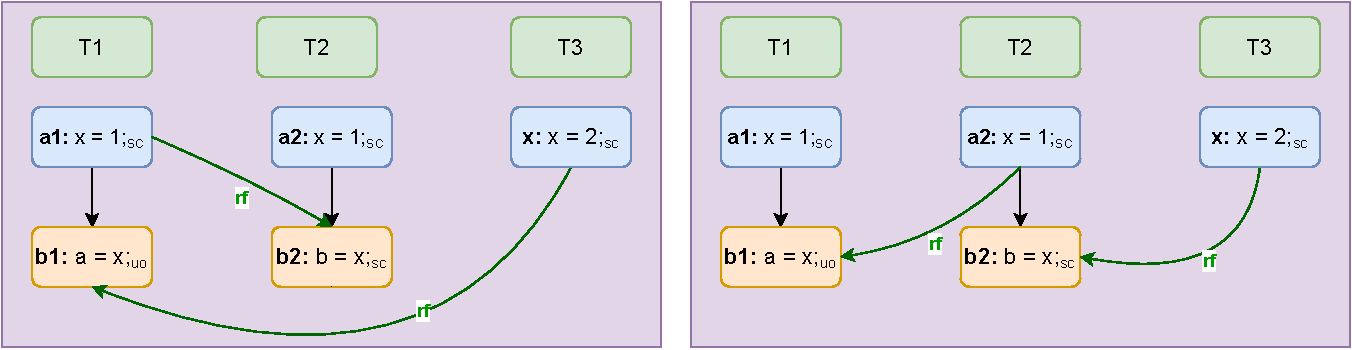
\includegraphics{Equivalence_Example.pdf}
            \caption{Example of program execution where resolving read orders does not keep read orders stable.}
            \label{read_ord:instability}
        \end{figure}

        In the above figure, notice that the read orders between $T_a$ and $T_b$ become incorrect once again while we resolve other implied read orders.
        
        \critic{red}{Perhaps also consider showing another example just to make them more assured of the fact that even prescribing an order in which we resolve these read orders, it does not matter.}

        \critic{red}{Show example where after fixing a read order and another, the previous one is present again.}

        Instead, what we will try to prove is \textbf{Forward Progress}; does resolving read orders eventually result in the irreflexivity condition to hold? 
        For this, we split our task into two parts, which are stated as two lemmas below. 
        Before that, we will introduce the notion of state here, to more formally state our requirement. 
        
        %Define the state here as a set of implied write orders and implied read orders.
        A state $S$ is a set of implied write orders and implied read orders.
        A transition from such a state to another involves swapping two thread identities, which may result in removal and addition of new implied write/read orders.
        For instance, transitioning from state $S$ to $S'$ after swapping threads $A$ and $B$ would be given as 
        \begin{align*}
            \reln{S}{(A,B)}{S'}.
        \end{align*}
        To depict multiple transitions of the above we will represent as $\reln{S}{*}{S'}$.
        \textit{Sound(S)}  depicts that the state $S$ respects Prop \ref{prop1}.
        
        
        \critic{red}{Show lemmas first, then the theorem. Prove the theorem first, assuming the lemmas hold. As the argument is quite intuitive. Then prove lemma 2 and show that it does not hold due to counter example. Then conclude that we cannot achieve optimality by resolving implied read orders. This would require changing the structure of the following content slightly.}

        Our first part is on the assumption that while resolving implied read orders, we do not encounter any incorrect implied write order. 
        %lemma to show that if an incorrect read order previously resolved is introduced by resolving another read order, then it implies the the currently resolved one remains unresolved before and after resolving the previous one
        \begin{lemma}
            \label{iro-stability}
            Consider a state $S$ such that $Sound(S) \ \wedge \ \reln{r_j}{iro}{r_i} \ \wedge \ i < j$.
            Consider state $S'$ after swapping threads $T_i$ and $T_j$ and assume that no incorrect implied write orders are introduced in doing so. 
            Consider also that $\reln{r_l}{iro}{r_k} \in S' \ \wedge \ k < l$.
            If we swap threads $T_l$ and $T_k$ giving resultant state $S''$, then 
            \begin{align*}
                \reln{r_j}{iro}{r_i} \in S'' 
                \Rightarrow
                \reln{r_l}{iro}{r_k} \in S
            \end{align*} 
        \end{lemma}

        \begin{proof}

            \critic{red}{Write this proof first. And while proving, show that one case is a counter example.}

            \begin{itemize}
                \item Case wise analysis.
                \item Infer different ordering relations to show that said implied read order is stable.
            \end{itemize}

        \end{proof}


        Our second lemma relaxes the assumption of the above lemma, thus allowing implied write orders to be incorrect. 
        This would mean, we will have to resolve them first, before once again resolving implied read orders.
        \begin{lemma}
            \label{iwo-unres-iro}
            Consider state $S$ such that $Sound(S) \ \wedge \ \reln{r_j}{iro}{r_i} \ \wedge \ i < j$.
            Consider state $S'$ that results after swapping threads $T_i$ and $T_j$. 
            Then if $\neg Sound(S')$, the new implied write orders introduced were not resolved in any previous state $S''$ such that $\reln{S''}{*}{S}$. 
        
            \critic{red}{The word resolved is important as it means there wasn't any step in state transition that involved swapping the two threads to resolve implied write order between them.}
        \end{lemma}


        \begin{proof}
            \begin{itemize}
                \item Case wise analysis
                \item Each case is proof by contradiction
                \item Main argument is the fixed order in which we fix the implied orders (writes first then reads)
            \end{itemize}    
        \end{proof}

        If the above lemmas hold, then we can resolve all such read orders to respect Def \ref{opt_cond}.
        The following theorem states this:
        %STOP HERE. 
        \begin{theorem}
            \label{fwdprog-iro}
            We can resolve all implied read orders to respect the irreflexivity constraints imposed on them.
        \end{theorem}

        \begin{proof}

            We begin the proof by considering a state $S$ representing the set of implied write/read orders we have in the current execution. 
            We further assume that all implied write orders have been resolved in $S$ ($Sound(S)$). 
            Now, we divide our analysis into two cases, which may take place while resolving read orders.
            For each case, we prove Forward Progress by that of contradiction.
            We try to see if we can reach the same state $S$ after resolving some orders, thus implying an endless cycle. 
            \begin{itemize}
                \item Case 1: If any incorrect implied write orders introduced in the process of resolving read orders. 

                    By Theorem \ref{iwo-sound}, we can resolve them. 
                    By Lemma \ref{iwo-unres-iro}, every implied write order introduced will be new.
                    Thus, by contradiction, we cannot retain the original state $S$ from which we resolve the same set of implied read orders. 

                \item Case 2: If no incorrect implied write orders introduced in the process of resolving read orders.

                    To retain the original state with a particular unresolved implied read order, we can only swap threads with incorrect implied read orders as per our assumption. 
                    By Lemma \ref{iro-stability}, obtaining a previously resolved iro as unresolved will in the process resolve another iro which remained stable while resolving the previous one.
                    By contradiction, this is not the same state as $S$. 
            \end{itemize}

            By Case 1 and 2, one cannot reach the same initial state.
            Because implied write/read orders are finite, the number of states are finite, and since we can only reach a state exactly once, 
            we can resolve all implied read orders in the process. 

            Hence proved.

        \end{proof}

        Surprisingly, Lemma \ref{iro-stability} does not hold. 
        The following example of an execution shows that we are stuck in a cycle resolving implied read orders.


        \begin{figure}
            \centering
            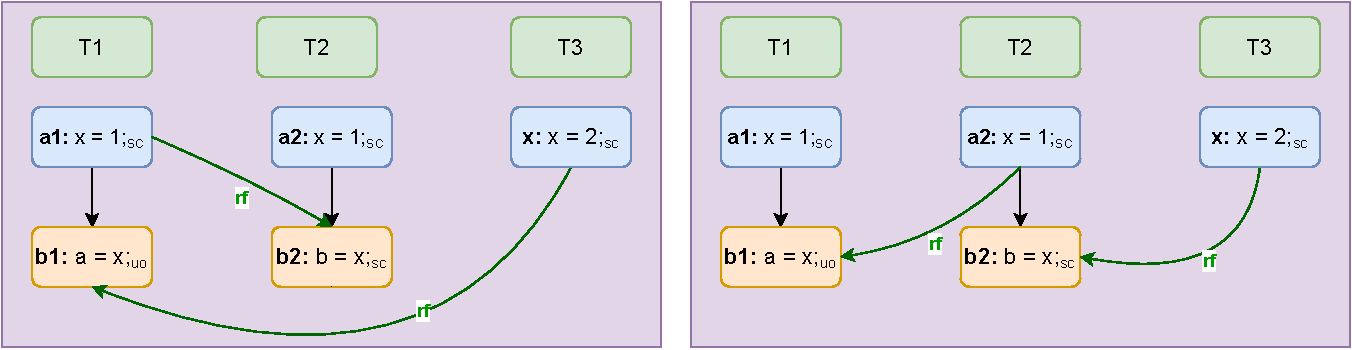
\includegraphics{Equivalence_Example.pdf}
            \caption{Set of executions, showing transitions while resolving read orders, which results in a cycle.}
            \label{iro:counter_example}
        \end{figure}

        In particular, from the above example, we note that:
        \begin{itemize}
            \item We cannot resolve all the implied read orders to respect our irreflexivity constraint for optimality.
            \item This is due to a cycle that is generated while resolving them using Prop \ref{iro-Rev}.
        \end{itemize}

        Thus, we cannot achieve optimality by resolving read orders. 

     
